% BASIC SETTINGS
\documentclass[a4paper,12pt]{article} % Set paper size and document type
\usepackage{lmodern} % Use a slightly nicer looking font
\usepackage{graphicx} % include figures

% Change margins - default margins are too broad
\usepackage[margin=20mm]{geometry}

% SOURCE CODE LISTING SETTINGS 
% https://en.wikibooks.org/wiki/LaTeX/Source_Code_Listings
\usepackage{listings}
\usepackage{color}

\definecolor{mygreen}{rgb}{0,0.6,0}
\definecolor{mygray}{rgb}{0.5,0.5,0.5}
\definecolor{mymauve}{rgb}{0.58,0,0.82}

\lstset{ %
  backgroundcolor=\color{white},   % choose the background color; you must add \usepackage{color} or \usepackage{xcolor}
  basicstyle=\footnotesize,        % the size of the fonts that are used for the code
  breakatwhitespace=false,         % sets if automatic breaks should only happen at whitespace
  breaklines=true,                 % sets automatic line breaking
  captionpos=b,                    % sets the caption-position to bottom
  commentstyle=\color{mygreen},    % comment style
  deletekeywords={...},            % if you want to delete keywords from the given language
  escapeinside={\%*}{*)},          % if you want to add LaTeX within your code
  extendedchars=true,              % lets you use non-ASCII characters; for 8-bits encodings only, does not work with UTF-8
  frame=single,	                   % adds a frame around the code
  keepspaces=true,                 % keeps spaces in text, useful for keeping indentation of code (possibly needs columns=flexible)
  keywordstyle=\color{blue},       % keyword style
  otherkeywords={*,...},           % if you want to add more keywords to the set
  numbers=left,                    % where to put the line-numbers; possible values are (none, left, right)
  numbersep=5pt,                   % how far the line-numbers are from the code
  numberstyle=\tiny\color{mygray}, % the style that is used for the line-numbers
  rulecolor=\color{black},         % if not set, the frame-color may be changed on line-breaks within not-black text (e.g. comments (green here))
  showspaces=false,                % show spaces everywhere adding particular underscores; it overrides 'showstringspaces'
  showstringspaces=false,          % underline spaces within strings only
  showtabs=false,                  % show tabs within strings adding particular underscores
  stepnumber=2,                    % the step between two line-numbers. If it's 1, each line will be numbered
  stringstyle=\color{mymauve},     % string literal style
  tabsize=2,	                   % sets default tabsize to 2 spaces
  title=\lstname                   % show the filename of files included with \lstinputlisting; also try caption instead of title
}

% PREPARE TITLE
\title{\textbf{Homework \#9 - Recursion}}
\author{Name: }
\date{} % Hide the date

% START DOCUMENT
\begin{document}

\maketitle % Insert the title

\section{Recursion}

You've probably seen code that looks like this before:

\vspace{5mm}
\begin{lstlisting}[language=C++]
for (int i = 10; i > 0; i--) {
	cout << i << endl;
}
\end{lstlisting}

\noindent
It's just a regular "for" loop that counts down from 10 to 1. Is there any other way to count from 10 to 1? Without a loop? And without just writing "cout" ten times? Turns out there is:

\vspace{5mm}
\lstinputlisting[language=C++, firstline=13]{simpleRecursion.cpp}

\noindent
If you take a close look at the function at the top, you'll notice that \textbf{it calls itself}! Functions are completely allowed to do this. You can write a C++ function that uses itself. This can be a difficult concept to understand at first, but it's very powerful and useful once you understand it.

\subsection{The Termination Condition}

Usually, recursive functions have an if/else inside that checks the value of an \textbf{argument} passed to the function. If the argument meets a certain condition, the recursion can continue (the function calls itself again), but with the argument changed (in this case, reduced by 1). If the argument does \textbf{not} meet the condition, the function does a "return". When this happens, we say the recursion has \textbf{terminated}. This means the function stops calling itself, and the computer goes "back up the call stack". That means that all the functions that were called finish their work and go back into our program's main() function. 

\subsection{Factorial}

Though it's hard to believe when you first see it, some algorithms are easiest to write if you write them recursively. A great example is \textbf{factorial}. You're probably familiar with factorial from math class. You write "factorial five" like this:

$$5!$$

\noindent
And it is solved like this:

$$5! = 5 \cdot 4 \cdot 3 \cdot 2 \cdot 1 = 120$$

\noindent
Imagine a recursive function to solve this. You could have a function that calls itself on 5, then 4, then 3....down to 1 then stops and \textbf{terminates the recursion}. Something like this:

\vspace{5mm}
\lstinputlisting[language=C++, firstline=13, lastline=20]{factorial.cpp}

\noindent
When the value "n" gets to 1, the function stops calling itself and just returns "1". All the functions above it would have done "n * factorial(n-1)", so the computer ended up doing something like this:

\vspace{5mm}
\begin{lstlisting}[language=C++]
factorial(5) * factorial(4) * factorial(3) * factorial(2) * factorial(1)
\end{lstlisting}

\noindent
Doing factorial(1) just returns a 1 into the function factorial(2), which does the math "2 * 1" and returns a "2" to factorial(3), which does "3 * 2" which returns the value "6" to factorial(4) which does "4 * 6" and returns "24" to factorial(5) which does "5 * 24" and then returns the final answer "120". So the recursion \textbf{collapses}, kind of like a folding telescope. To illustrate this for you, imagine a program that did "cout \textless \textless \space num;" and then called itself on "num + 1", stopping when "num == 4". If we started it at "0" we'd get something like this when it ran:

\vspace{5mm}
% Insert a figure with an image
\begin{figure}[!ht]
  \centering
  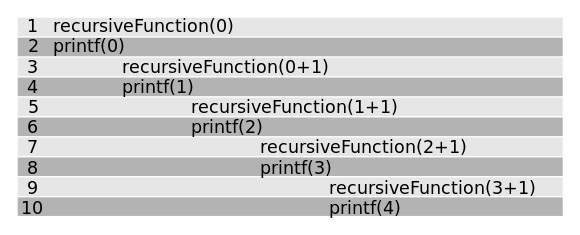
\includegraphics[width=0.7\textwidth]{recursion.png}
  \caption{A Simple Recursion}
\end{figure}

\section{Now You Try}

There is a famous \textbf{series} (a set of numbers counting up or down) in mathematics called the \textbf{Fibonacci series}. It goes like this:

\begin{verbatim}
1 1 2 3 5 8 13 21 34 55 89 144...
\end{verbatim}

\noindent
Can you see a pattern here? $0+1 = 1$, the next number in the series. Then $1+1 = 2$, the next number. $1 + 2 = 3$, $2 + 3 = 5$, $3 + 5 = 8$, and so on. Try to write a \textbf{recursive} C++ program that print out this series. You should have a function in your code that looks like this:

\vspace{5mm}
\begin{lstlisting}[language=C++]
void fibonacci(int a, int b, int n){
	// YOUR CODE HERE
}
 \end{lstlisting}
 
 \noindent
 If you wanted the first 12 numbers, you'd set "a" and "b" to be "0" and "1" and you'd set "n" to "12". Like this:
 
 \vspace{5mm}
\begin{lstlisting}[language=C++]
 int main() {

    cout << "The first 12 Fibonacci numbers: " << endl;
    fibonacci(0, 1, 12);
    
    return 0;
}
 \end{lstlisting}

\noindent
Which would print out:

\begin{verbatim}
1 1 2 3 5 8 13 21 34 55 89 144
\end{verbatim}

\noindent
Think about how the 3 arguments to fibonacci should \textbf{change} each time the function is called. Think about what number the fibonacci function should print out each time it is called. Think about what should happen when "n == 0". Have a look at the files \textbf{factorial.cpp} and \textbf{simpleRecursion.cpp} for inspiration.

\end{document}